\documentclass[11pt]{jarticle}

\usepackage[dvipdfmx]{graphicx}
\usepackage{listings}
\usepackage{url}

\lstset{
    basicstyle={\ttfamily\small}, %書体の指定
    frame=tRBl, %フレームの指定
    framesep=10pt, %フレームと中身(コード)の間隔
    breaklines=true, %行が長くなった場合の改行
    linewidth=16cm, %フレームの横幅
    lineskip=-0.5ex, %行間の調整
    tabsize=2 %Tabを何文字幅にするかの指定
}

\setlength{\oddsidemargin}{-6.35mm}
\setlength{\textwidth}{171.9mm}

\begin{document}

\title{画像処理実験 第8回}
\author{09430565\\大橋虎ノ介}
\date{\number\year 年\number\month 月\number\day 日}
\maketitle

\section{概要}

本報告書では,8回の実験を通して自動パノラマ合成プログラムを作成した結果を
報告する.
第1回はコンピュータ内での画像の扱いと簡単な画像処理を学んだ.
第2回から第7回までは自動パノラマ合成プログラムで使用する以下の表に示す機能を
を実装した.

第8回ではこれまで実装した機能をつなぎ合わせ,自動パノラマ合成プログラムを
作成する.
パノラマ画像の作成には,コマンドライン上で\\
{\bf 今回作った実行ファイル.exe 第1画像 第2画像}\\
を実行することでパノラマ画像が作成できることを目指す.

\begin{table}[h]
    \begin{tabular}{lll}
         & 機能 \\ \hline
        第2回 & 3x3行列の積を計算する, 画像の幾何学変換 \\
        第3回 & 対応点から射影変換行列を求める \\
        第4回 & 特徴点の自動検出を行う \\
        第5回 & 画像全体で特徴的な点を選択する \\
        第6回 & 類似度を計算し特徴点対を選択する \\
        第7回 & 特徴点対の中から正しい特徴点対を選択する \\
        
    \end{tabular}
\end{table}

\section{講義時間内に達成できなかった課題}

\subsection{第2回レポート}

\subsubsection{解説ページのprocess関数と同様の処理をC言語で実装する}

process関数と同様の処理をするImageImageProjectionAlpha関数を示す.
process関数により出力される画像(左)とImageImageProjectionAlpha関数に
より出力される画像(右)を示す.

\begin{lstlisting}
void ImageImageProjectionAlpha(Image* id, Image* is, double a[3][3], double alpha) {
    int x, y, u, v;
    double r;
    for (y = 0; y < id->H; y++) for (x = 0; x < id->W; x++) {
        r = 1 / (a[2][0] * x + a[2][1] * y + a[2][2]);
        u = r * (a[0][0] * x + a[0][1] * y + a[0][2]);
        v = r * (a[1][0] * x + a[1][1] * y + a[1][2]);
        if (isInsideImage(is, u, v)) {
            IElem(id, x, y, 0) += IElem(is, u, v, 0) * alpha,
            IElem(id, x, y, 1) += IElem(is, u, v, 1) * alpha,
            IElem(id, x, y, 2) += IElem(is, u, v, 2) * alpha;
        }
    }
}
\end{lstlisting}

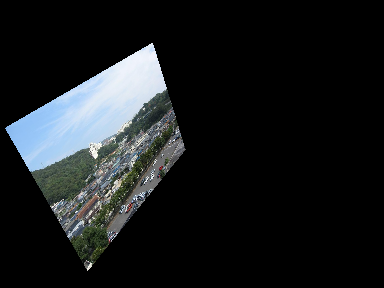
\includegraphics[scale=.6]{./img/dai2js.png}
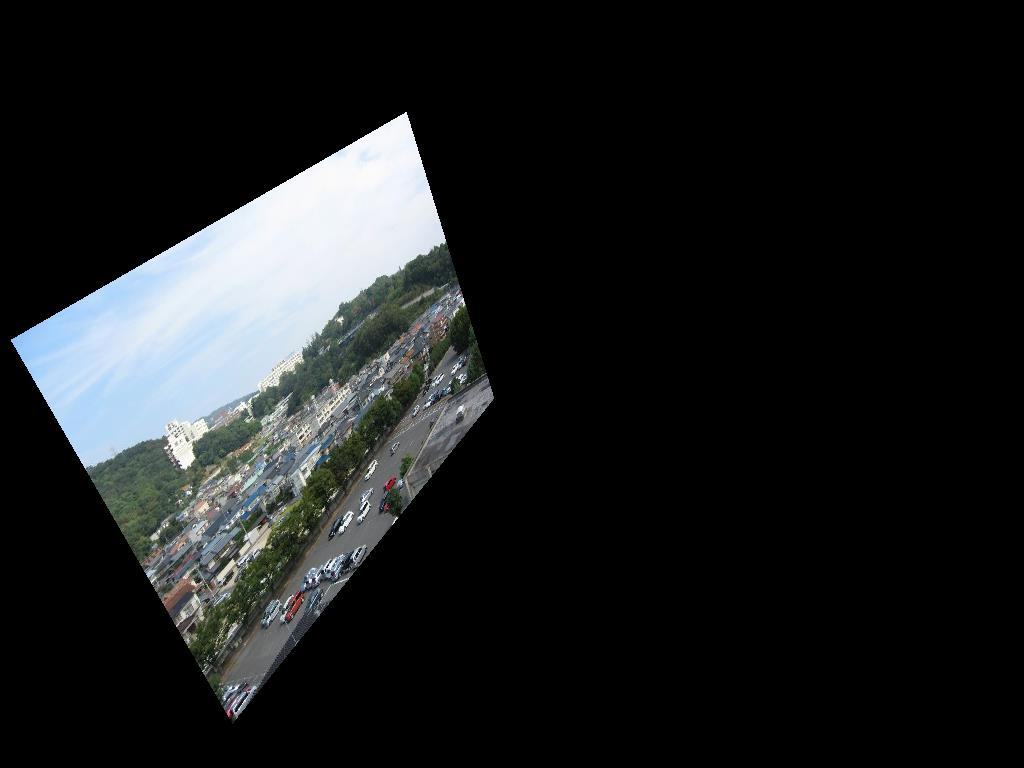
\includegraphics[scale=.3]{./img/c_henkan.jpg}

\subsubsection{3x3行列の積を計算するmult33関数を実装し,画像を合成する.}

第2回レポート作成時はImageMagickがエラーをはいて一部が欠けて,色がおかしい画像が出力されていた.
Visual Studioの警告を出さないように設定すると,正しい画像が出力されるようになった.

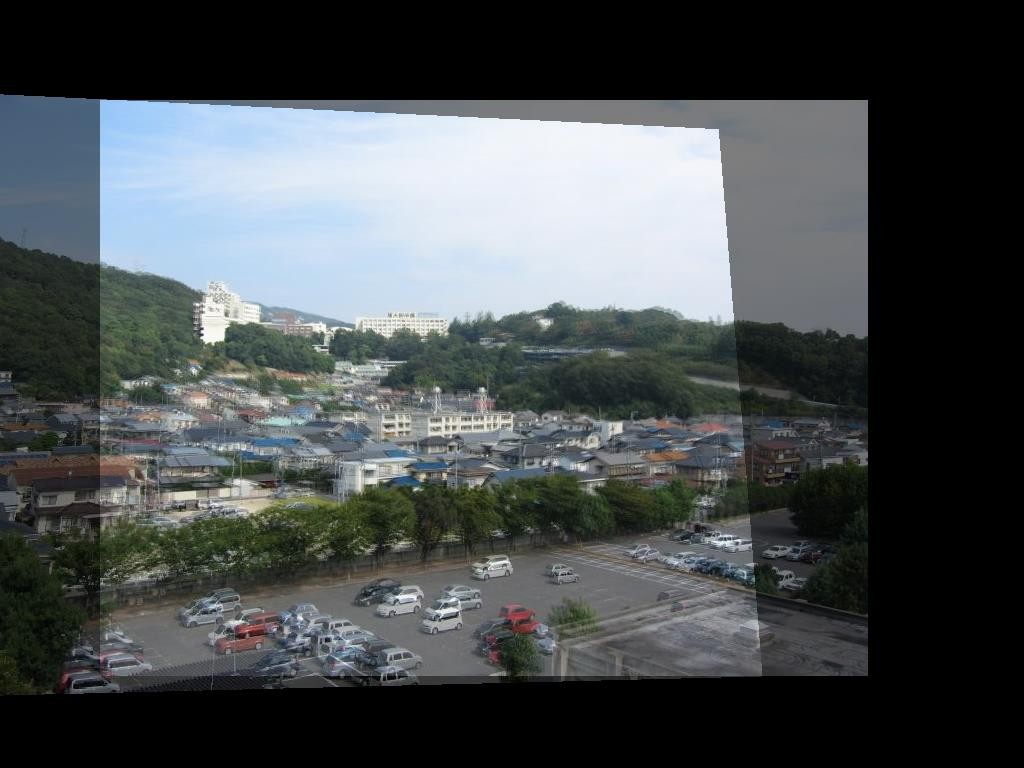
\includegraphics[scale=.6]{./img/dai2out.jpg}

\section{自動パノラマ画像合成プログラム}

2枚の画像を自動で合成するプログラムを作成した.
出力画像の大きさは,今までは定数で固定していたが,様々な大きさの画像に
対応するために第一画像の大きさから定数倍することにした.

\section{各回で作った機能}

ここでは,自動パノラマ合成プログラムに必要な関数を報告する.

\subsection{第2回 3x3行列の積を計算する,画像の幾何学変換}

3x3行列の積を計算するmult33関数と画像を幾何学変換する
ImageImageProjectionAlpha関数を以下のように実装した.

\begin{lstlisting}
    void mult33(double d[3][3], double a[3][3], double b[3][3]) {
        int x, y, i;
    
        for (y = 0; y < 3; y++)
            for (x = 0; x < 3; x++) {
                d[y][x] = 0;
                for (i = 0; i < 3; i++){
                    d[y][x] += a[y][i] * b[i][x];
                }
            }
    }
\end{lstlisting}

\begin{lstlisting}
    void ImageImageProjectionAlpha(Image* id, Image* is, double a[3][3], double alpha) {
        int x, y, u, v;
        double r;
        for (y = 0; y < id->H; y++) for (x = 0; x < id->W; x++) {
            r = 1 / (a[2][0] * x + a[2][1] * y + a[2][2]);
            u = r * (a[0][0] * x + a[0][1] * y + a[0][2]);
            v = r * (a[1][0] * x + a[1][1] * y + a[1][2]);
            if (isInsideImage(is, u, v)) {
                IElem(id, x, y, 0) += IElem(is, u, v, 0) * alpha,
                IElem(id, x, y, 1) += IElem(is, u, v, 1) * alpha,
                IElem(id, x, y, 2) += IElem(is, u, v, 2) * alpha;
            }
        }
    }
\end{lstlisting}

\subsection{第3回 対応点から射影変換行列を求める}

最小二乗法によって,対応点から射影変換を求めるcalcm10関数を以下のように実装した.
ここでMatrixQRDecompColMajorはQR分解,MatrixSimeqLrは後退代入をする関数である.
なお,第8回ではcalcHomography関数として呼び出され,関数内で定義していた
*cmA, *vt, *mtR, *tmpは引数として受け取る.

\begin{lstlisting}
void MatrixQRDecompColMajor(Matrix* mtR, Matrix* mt) {
    // Gram-Schmidt orthonormalization (R and Q)
    double t, * aT[] = { Row(mt,0), Row(mt,1), Row(mt,2), Row(mt,3), Row(mt,4), Row(mt,5), Row(mt,6), Row(mt,7) };
    int W = mt->W;
    MatrixClear(mtR);

    int i, j;
    for (i = 0; i < 8; i++) {
        for (j = 0; j < i; j++) {
            Elem(mtR, j, i) = t = VP(aT[j], aT[i], W);
            VSA(aT[i], aT[j], -t, W);
        }
        Elem(mtR, i, i) = t = sqrt(VP(aT[i], aT[i], W));
        VSS(aT[i], 1 / t, W);
    }

}

void MatrixSimeqLr(Matrix* mtB, Matrix* mtR) {
    // B = B L^{-1}
    double* B = Row(mtB, 0);
    double tmp;
    int i, j;
    for (i = 7; i >= 0; i--) {
        tmp = B[i];
        for (j = i+1; j <= 7; j++) {
            tmp -= B[j] * Elem(mtR, i, j);
        }
        B[i] = tmp / Elem(mtR, i, i);
    }
}

void calcm10(double m10[3][3]) {
    Matrix* cmA, * vt, * mtR, * tmp;
    int i,j;

    double w[][4] = { // (x,y,u,v)
        99,210,219,226,
        195,519,314,528,
        355,506,473,518,
        615,439,743,453,
    };

    cmA = MatrixAlloc(8, 8);
    vt = MatrixAlloc(1, 8);

    // create A (col-major)
    for (i = 0; i < 4; i++) {
        Elem(cmA, 0, i * 2) = w[i][0];
        Elem(cmA, 1, i * 2) = w[i][1];
        Elem(cmA, 2, i * 2) = 1;
        Elem(cmA, 3, i * 2) = 0;
        Elem(cmA, 4, i * 2) = 0;
        Elem(cmA, 5, i * 2) = 0;
        Elem(cmA, 6, i * 2) = -w[i][0] * w[i][2];
        Elem(cmA, 7, i * 2) = -w[i][1] * w[i][2];
        Elem(cmA, 0, i * 2 + 1) = 0;
        Elem(cmA, 1, i * 2 + 1) = 0;
        Elem(cmA, 2, i * 2 + 1) = 0;
        Elem(cmA, 3, i * 2 + 1) = w[i][0];
        Elem(cmA, 4, i * 2 + 1) = w[i][1];
        Elem(cmA, 5, i * 2 + 1) = 1;
        Elem(cmA, 6, i * 2 + 1) = -w[i][0] * w[i][3];
        Elem(cmA, 7, i * 2 + 1) = -w[i][1] * w[i][3];
        Elem(vt, 0, i * 2) = w[i][2];
        Elem(vt, 0, i * 2 + 1) = w[i][3];
    }

    // solve Least-squares equation
    mtR = MatrixAlloc(8, 8);
    MatrixQRDecompColMajor(mtR, cmA);
    tmp = MatrixAlloc(1, 8);
    MatrixMultT(tmp, vt, cmA);
    MatrixSimeqLr(tmp, mtR);
    MatrixPrint(tmp);
    for (i = 0; i < 3; i++) for (j = 0; j < 3; j++) {
        if (i == 2 && j == 2) {
            m10[i][j] = 1;
        }
        else {
            m10[i][j] = tmp->data[i*3+j];
        }
    }
}
\end{lstlisting}

\subsection{第4回 特徴点の自動検出を行う}

ImageFeature関数は各画素ごとに特徴点らしさの計算を行う.
CalcSmallerEigenValue関数は,2x2の行列の小さい方の固有値を計算する.
この関数は,短径領域での和を2段階で計算することで,約7分の1の時間短縮を
果たした.

\begin{lstlisting}
    double CalcSmallerEigenValue(double a, double b, double c, double d) {
        double x = ((a + d) - sqrt((a + d) * (a + d) 
                    - 4 * (a * d - b * c))) / 2;
        return x;
    }
    
    void ImageFeature(Matrix* im2, Image* im) {
        int x, y, u, v, W = 7;
        double ix, iy;
        Matrix* tmpxx,*tmpxy,*tmpyy;
        tmpxx = MatrixAlloc(im2->W, im2->H);
        tmpxy = MatrixAlloc(im2->W, im2->H);
        tmpyy = MatrixAlloc(im2->W, im2->H);
        for (y = W + 1; y < im->H - W - 1; y++) for (x = W + 1; x < im->W - W - 1; x++) {
            double ixx, ixy, iyy;
            ixx = iyy = ixy = 0;
            for (u = -W; u <= W; u++) {
                ix = IElem(im, x + u + 1, y, 1) - IElem(im, x + u - 1, y, 1);
                iy = IElem(im, x + u, y + 1, 1) - IElem(im, x + u, y - 1, 1);
                ixx += ix * ix;
                ixy += ix * iy;
                iyy += iy * iy;
            }
            DElem(tmpxx, x, y) = ixx;
            DElem(tmpxy, x, y) = ixy;
            DElem(tmpyy, x, y) = iyy;
        }

        for (y = W + 1; y < im->H - W - 1; y++) for (x = W + 1; x < im->W - W - 1; x++) {
            double ixx, ixy, iyy;
            ixx = iyy = ixy = 0;
            for (v = -W; v <= W; v++) {
                ixx += DElem(tmpxx, x, y + v);
                ixy += DElem(tmpxy, x, y + v);
                iyy += DElem(tmpyy, x, y + v);
            }
            DElem(im2, x, y) = CalcSmallerEigenValue(ixx, ixy, ixy, iyy);
        }
    }
\end{lstlisting}

\subsection{第5回 画像全体で特徴的な点を選択する}

MatrixLocalMax関数は,第4回で計算した特徴点らしさの行列を受け取り,
画像全体で特徴点となりうる点の座標をw[][2]に格納しその数を返す.
この関数は,短径領域での和を2段階で計算することで,約2分の1の時間短縮を
果たした.

\begin{lstlisting}
    int MatrixLocalMax(int w[][2], Matrix* im2) {
        int x, y, u, v, W = 7, n = 0, a;
        Matrix* tmp;
        tmp = MatrixAlloc(im2->W, im2->H);
        for (y = W + 1; y < im2->H - W - 1; y++) for (x = W + 1; x < im2->W - W - 1; x++) {
            DElem(tmp, x, y) = -1;
            for (v = -W; v <= W; v++) {
                if (DElem(tmp, x, y) < DElem(im2, x, y + v)) {
                    DElem(tmp, x, y) = DElem(im2, x, y + v);
                }
            }
        }
        for (y = W + 1; y < im2->H - W - 1; y++) for (x = W + 1; x < im2->W - W - 1; x++) {
            for (u = -W; u <= W; u++) {
                if (DElem(tmp, x, y) < DElem(im2, x + u, y)) DElem(tmp, x, y) = DElem(im2, x + u, y);
            }
            // 最大値が DElem(im2,x,y) と等しいなら,(x,y) を特徴点として記録する. 
            if (DElem(tmp, x, y) == DElem(im2, x, y)) {
                a = n; if (n < Max) n++;
                for (; a > 0 && DElem(im2, w[a - 1][0], w[a - 1][1]) < DElem(im2, x, y); a--) {//InsertionSort
                    w[a][0] = w[a - 1][0];
                    w[a][1] = w[a - 1][1];
                }
                w[a][0] = x;
                w[a][1] = y;
            }
        }
        return n; // 記録した点の数 
    }
\end{lstlisting}

\subsection{第6回 類似度を計算し特徴点対を選択する}

matchMethod1関数は,類似度の表mtから同一の物体を指す特徴点の
対をw[][4]へ格納する.

\begin{lstlisting}
    int matchMethod1(double w[][4], Matrix* mt,
        Image* im, int x1[][2], int N1,
        Image* im2, int x2[][2], int N2) {
        int i, j, k, ti, tj, n, loop;
        if (N1 < N2) {
            loop = N1;
        }
        else {
            loop = N2;
        }
        for (n = 0; n < loop; n++) {
            double sm = INFINITY, t;
            for (i = 0; i < N1; i++) for (j = 0; j < N2; j++) {
                t = Elem(mt, i, j);
                if (sm > t) sm = t, ti = i, tj = j;
            }
            /*printf("%d,%d,%d,%d,\n",
                x1[ti][0], x1[ti][1],
                x2[tj][0], x2[tj][1]);*/
            w[n][0] = x1[ti][0];
            w[n][1] = x1[ti][1];
            w[n][2] = x2[tj][0];
            w[n][3] = x2[tj][1];
            for (k = 0; k < N1; k++) Elem(mt, k, tj) = INFINITY;
            for (k = 0; k < N2; k++) Elem(mt, ti, k) = INFINITY;
        }
        return n;
    }
\end{lstlisting}

\subsection{第7回 特徴点対の中から正しい特徴点対を選択する}

第6回で得た特徴点の組から,正しい特徴点対を選ぶ.
ransac関数は特徴点対からランダムに4つ選び,
射影変換行列と正しさを計算する.
ここでは,射影変換行列を満たす
特徴点対の数を正しさの指標とし,スコアが高かった
射影変換行列をbestH[3][3]に格納する.

\begin{lstlisting}
void ransac(double bestH[3][3], double w[][4]) {
    int best_score = 0;
    int rndAry[MAX];
    int score;
    Matrix* cmA, * vt, * mtR, * tmp;
    cmA = MatrixAlloc(8, 8);
    vt = MatrixAlloc(1, 8);
    mtR = MatrixAlloc(8, 8);
    tmp = MatrixAlloc(1, 8);
    initRndAry(rndAry);
    for (int trial = 0; trial < TRIAL; trial++) {
        double H[3][3]; // 選んだ4点から計算される変換行列の置き場
        chooseFourNumbers(rndAry);
        calcHomography(H, w, rndAry, cmA, vt, mtR, tmp);
        score = calcScore(H, w);
        if (best_score < score) {
            printf("score: %d\n", score);
            for (int i = 0; i < 3; i++) for (int j = 0; j < 3; j++) {
                bestH[i][j] = H[i][j];
            }
            best_score = score;
        }
    }

}
\end{lstlisting}

\section{自動パノラマ合成プログラム}

\begin{lstlisting}
    int main(int ac, char** av) {
        Image* im, * im2, * id;
        /*
            im:  第1画像を格納
            im2: 第2画像を格納
            id:  出力画像の格納
        */
        Matrix* mt, * imf, * im2f;
        /*
            mt:  SSDテーブルを格納
            imf: 第1画像の特徴点画像を格納
            im2f:第2画像の特徴点画像を格納
        */
        int x1[MAX][2], x2[MAX][2], N1, N2;
        /*
            x1:  第1画像の特徴点座標を格納
            x2:  第2画像の特徴点座標を格納
            N1:  第1画像の特徴点座標の個数を格納
            N2:  第2画像の特徴点座標の個数を格納
        */
        double m0d[][3] = {
            1,0,-100,
            0,1,-100,
            0,0,1
        };
    
        if (ac < 3) return 1;
    
        im = ImageRead(av[1]);
        im2 = ImageRead(av[2]);
        imf = MatrixAlloc(im->H, im->W);
        im2f = MatrixAlloc(im2->H, im2->W);
        id = ImageAlloc(im->W*1.2, im->H*1.1);
        ImageFeature(imf, im);                             
        ImageFeature(im2f, im2);
        //特徴点の検出(実験第4回)

        N1 = MatrixLocalMax(x1, imf);
        N2 = MatrixLocalMax(x2, im2f);                      
        //画像全体で特徴的な点を選び出す(実験第5回)
    
        mt = MatrixAlloc(N1, N2);       
        calcSSDtable(mt, im, x1, N1, im2, x2, N2);          
        //類似度を計算しSSDテーブルを作成する(実験第6回)
    
        double w[MAX][4];
        int nm;
        nm = matchMethod1(w, mt, im, x1, N1, im2, x2, N2);  
        //SSDテーブルから特徴点対を選ぶ(実験第6回)

        double H[3][3];
        ransac(H, w);                                       
        //RANSACで正しい特徴点対4組とそれに対応する射影変換行列を計算する(実験第7回,実験第3回)
    
    
        ImageImageProjectionAlpha(id, im, m0d, .5);         
        //第1画像を出力画像に書き込む
        double m1d[3][3];
        mult33(m1d, H, m0d);                                
        //行列の積を求める(実験第2回)
        ImageImageProjectionAlpha(id, im2, m1d, .5);        
        //第2画像を出力画像に書き込む
    
        ImageWrite("out.jpg", id);
        return 0;
    }
\end{lstlisting}

\section{自分で撮影した画像の合成}

作成した自動パノラマ合成プログラムに自分で撮影した画像を入力したところ,
正しく合成されるものとされないものがあった.まず,正しく合成された例を
示す.以下二つの画像を入力した結果,正しいパノラマ画像が得られた.


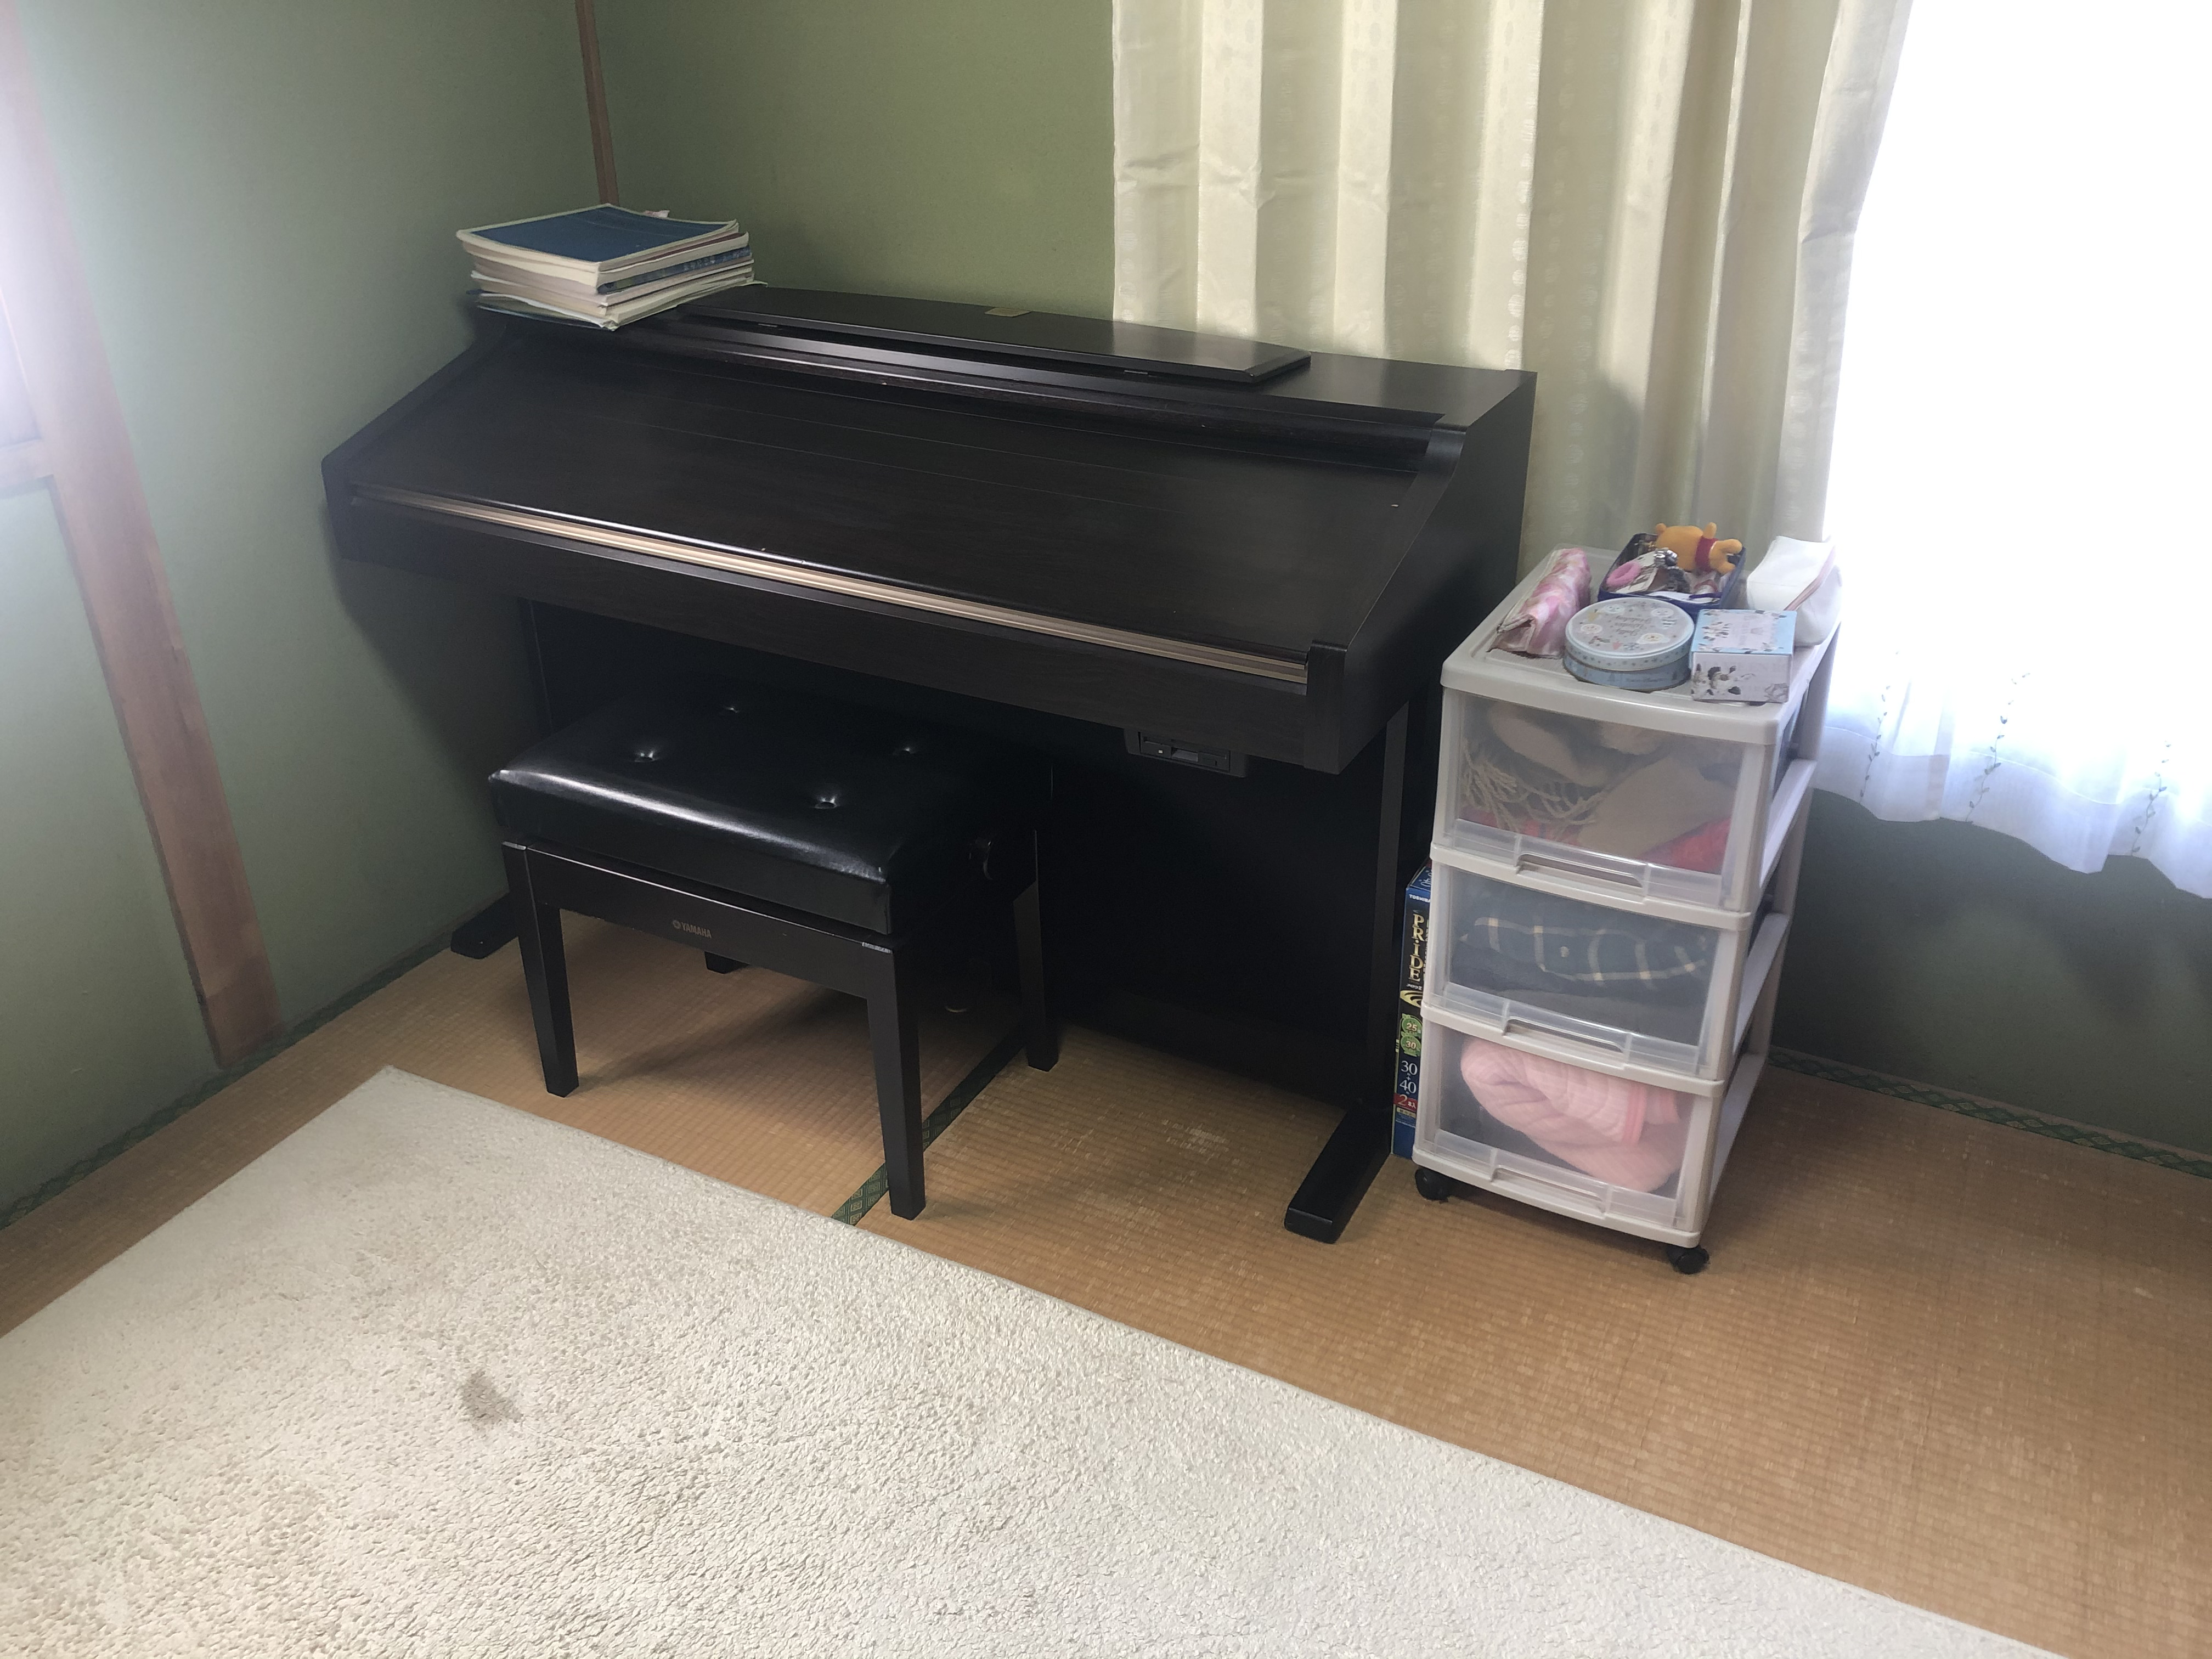
\includegraphics[scale=.055]{./img/piano0.jpg}
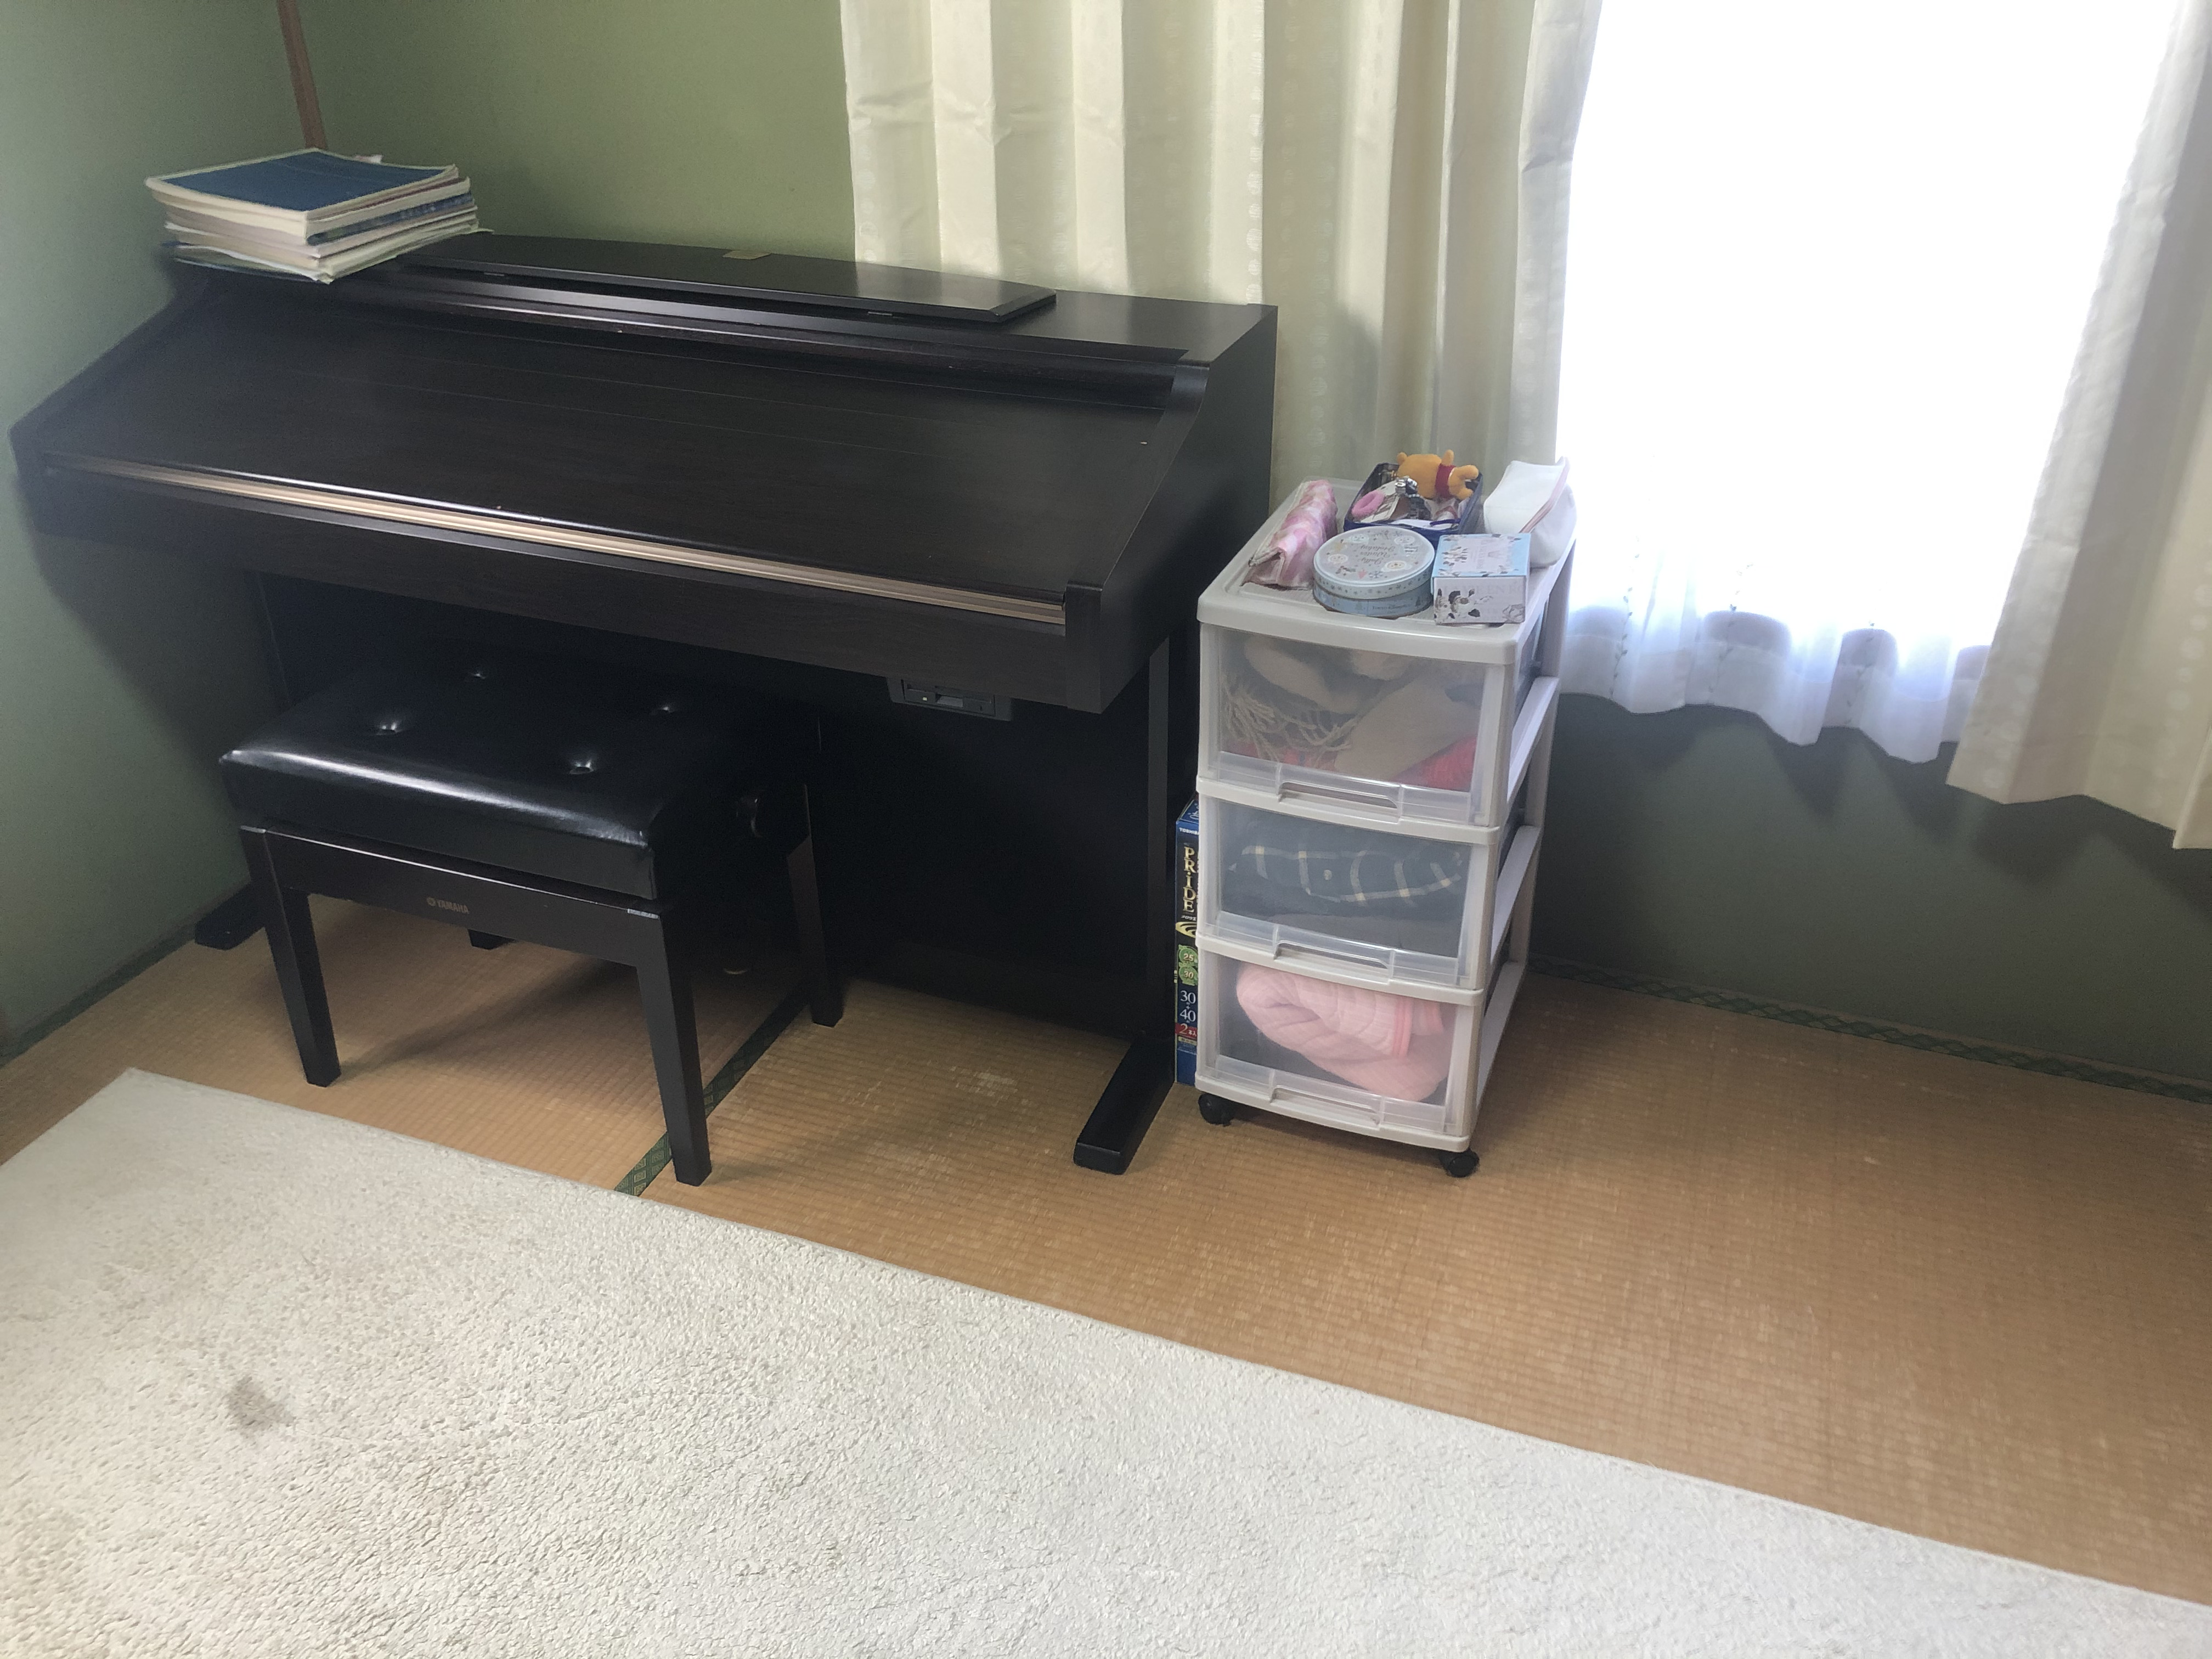
\includegraphics[scale=.055]{./img/piano1.jpg}

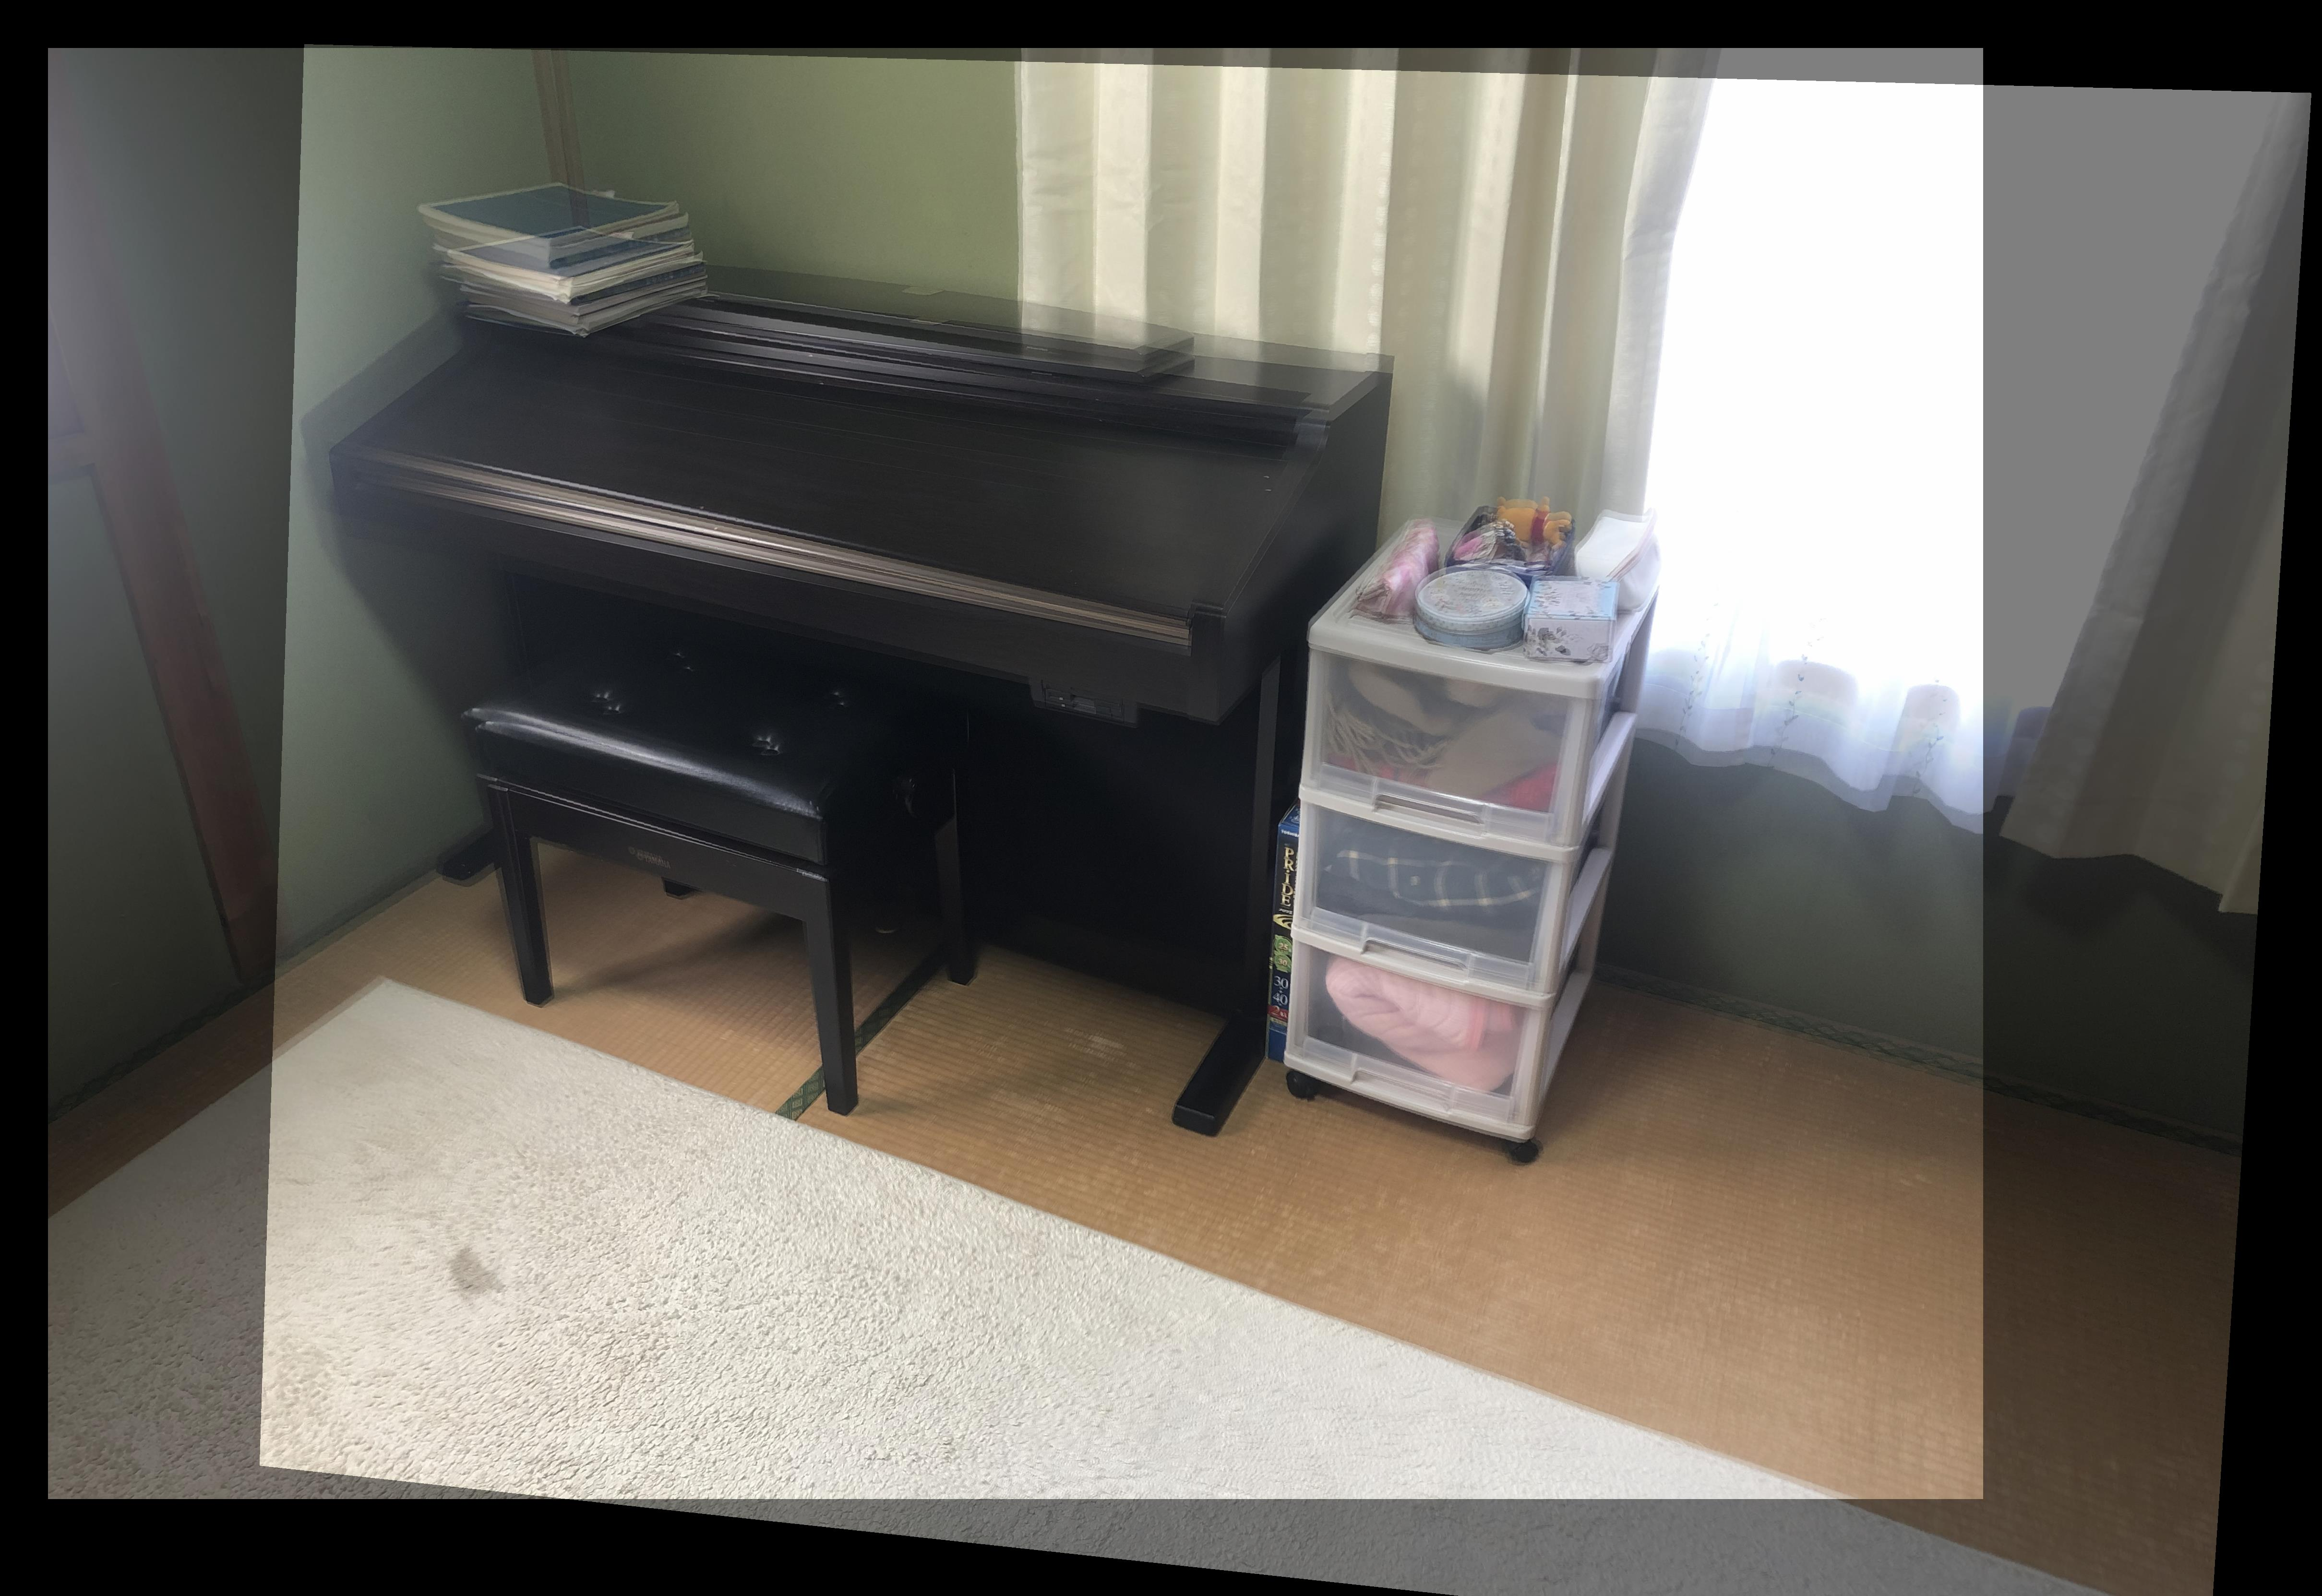
\includegraphics[scale=.11]{./img/pianoout.jpg}

次に正しく合成されなかった例を示す.


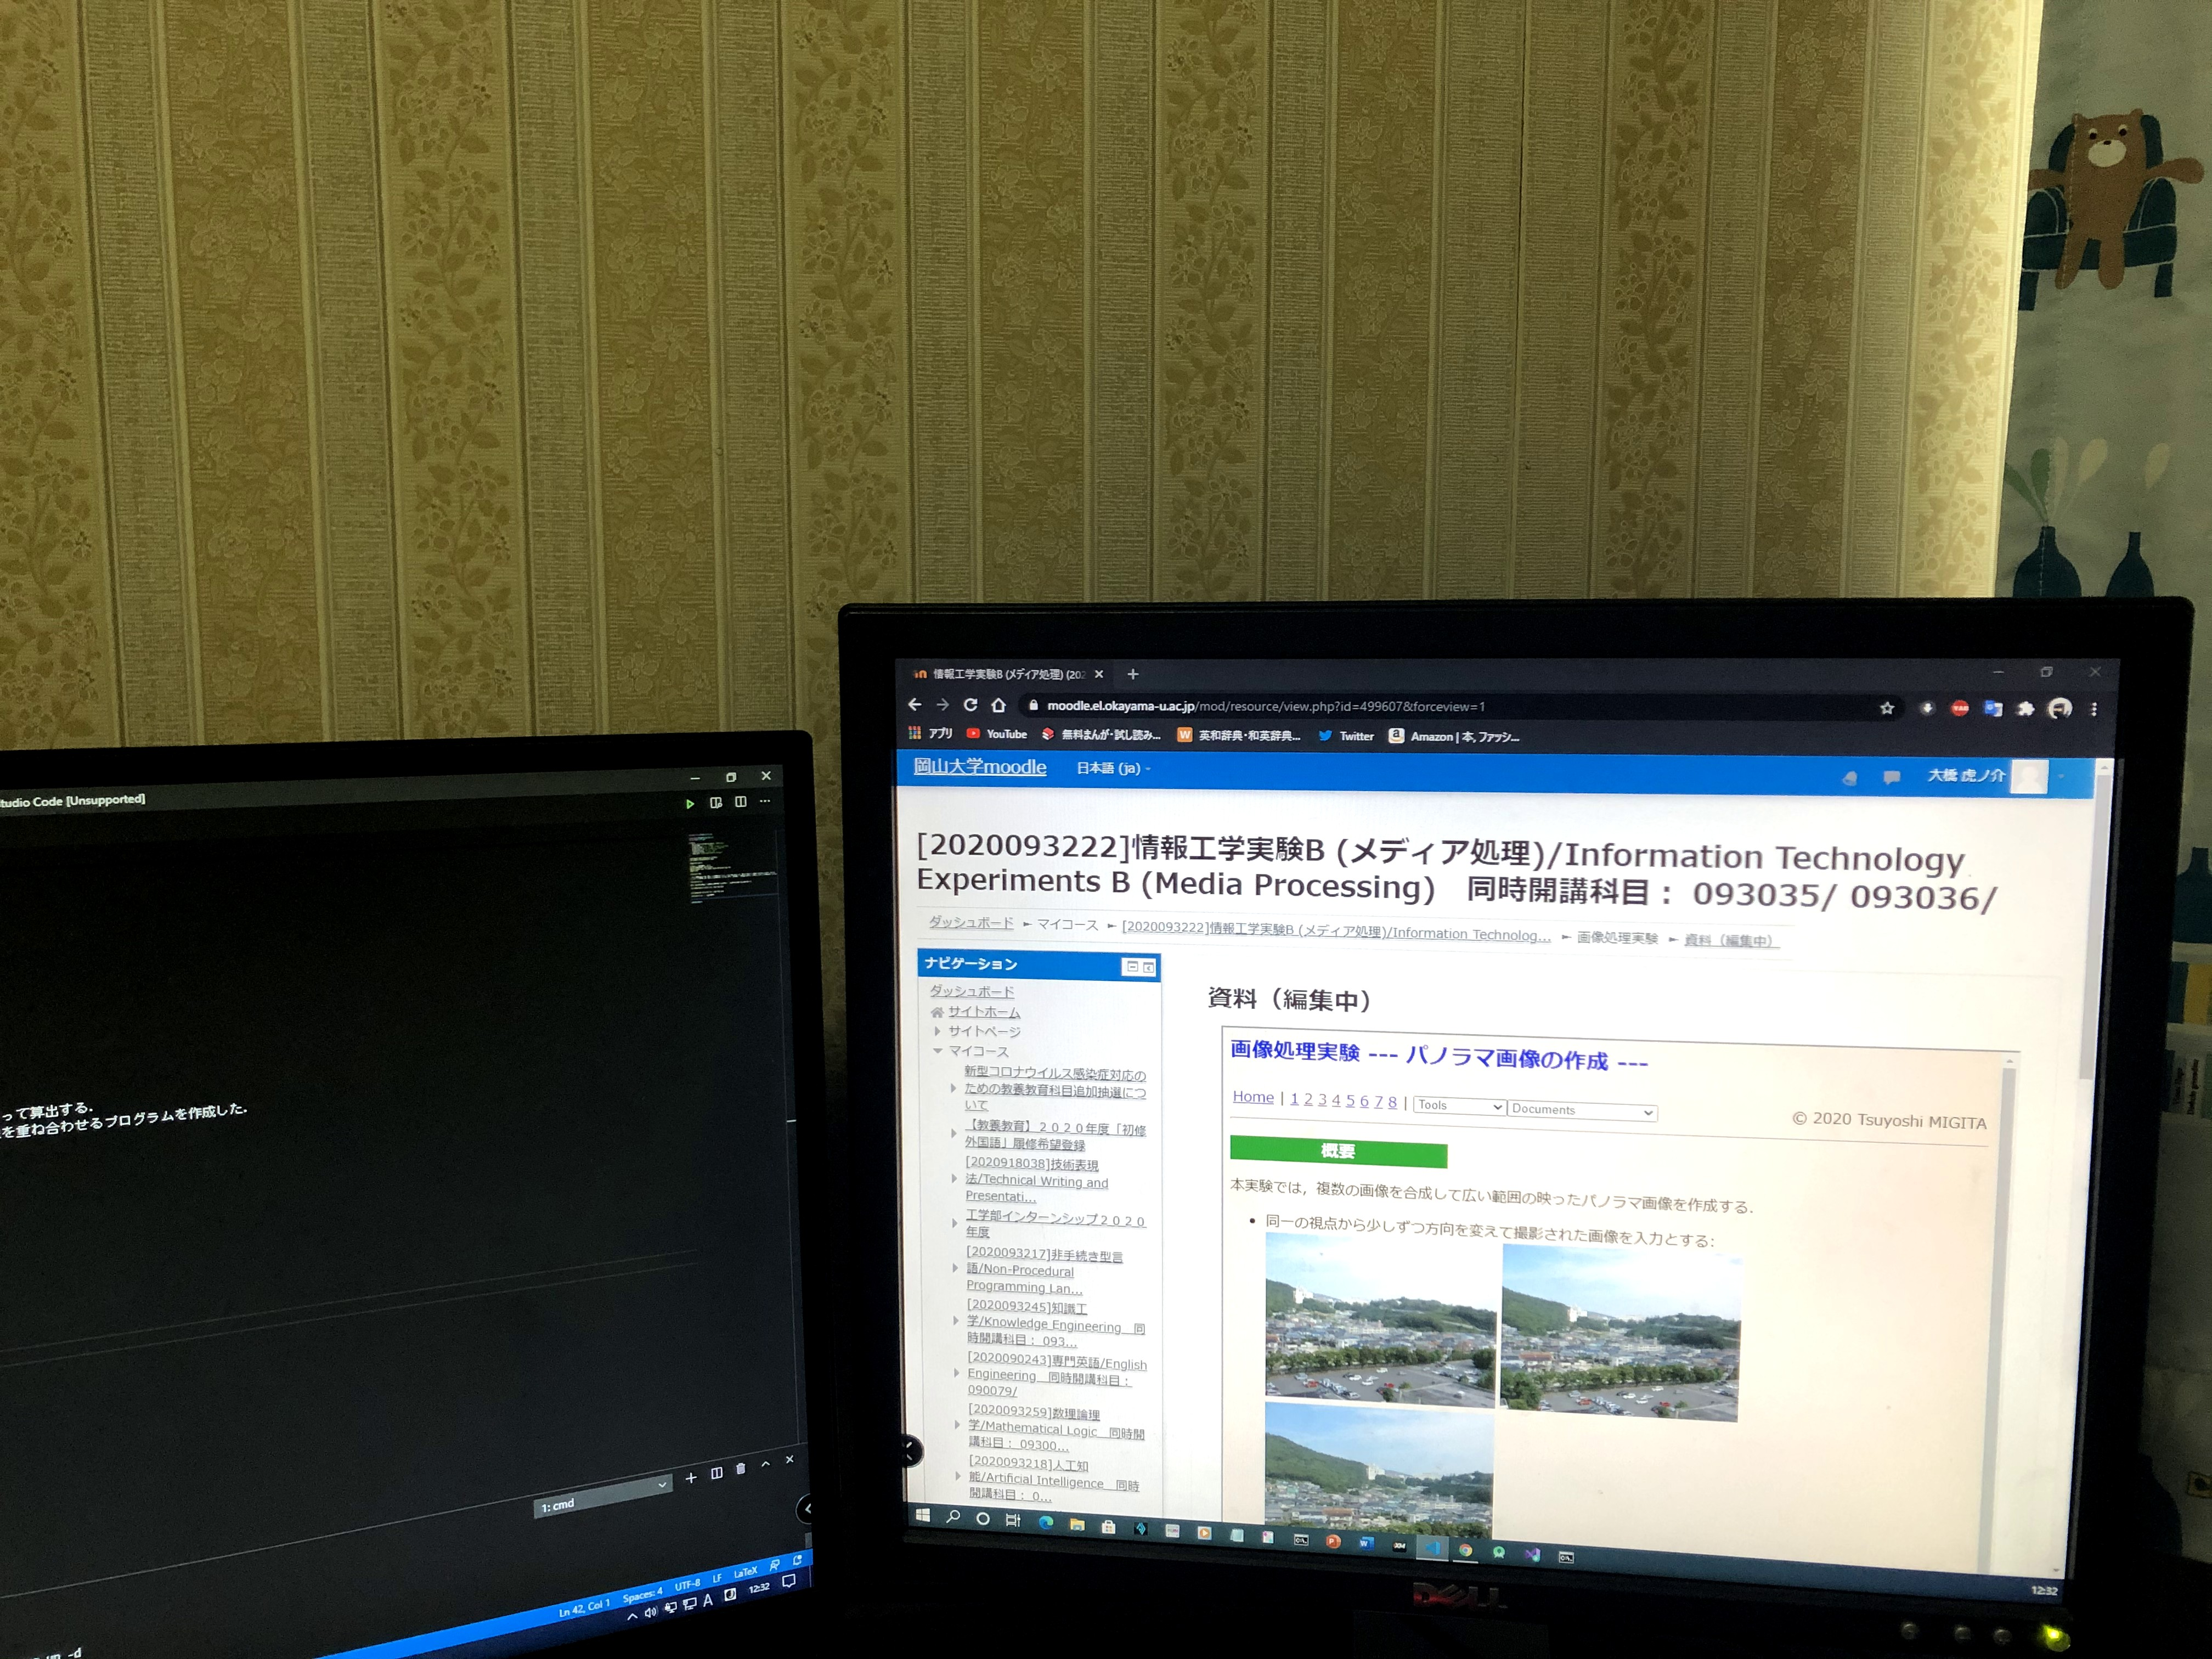
\includegraphics[scale=.055]{./img/desktop0.JPG}
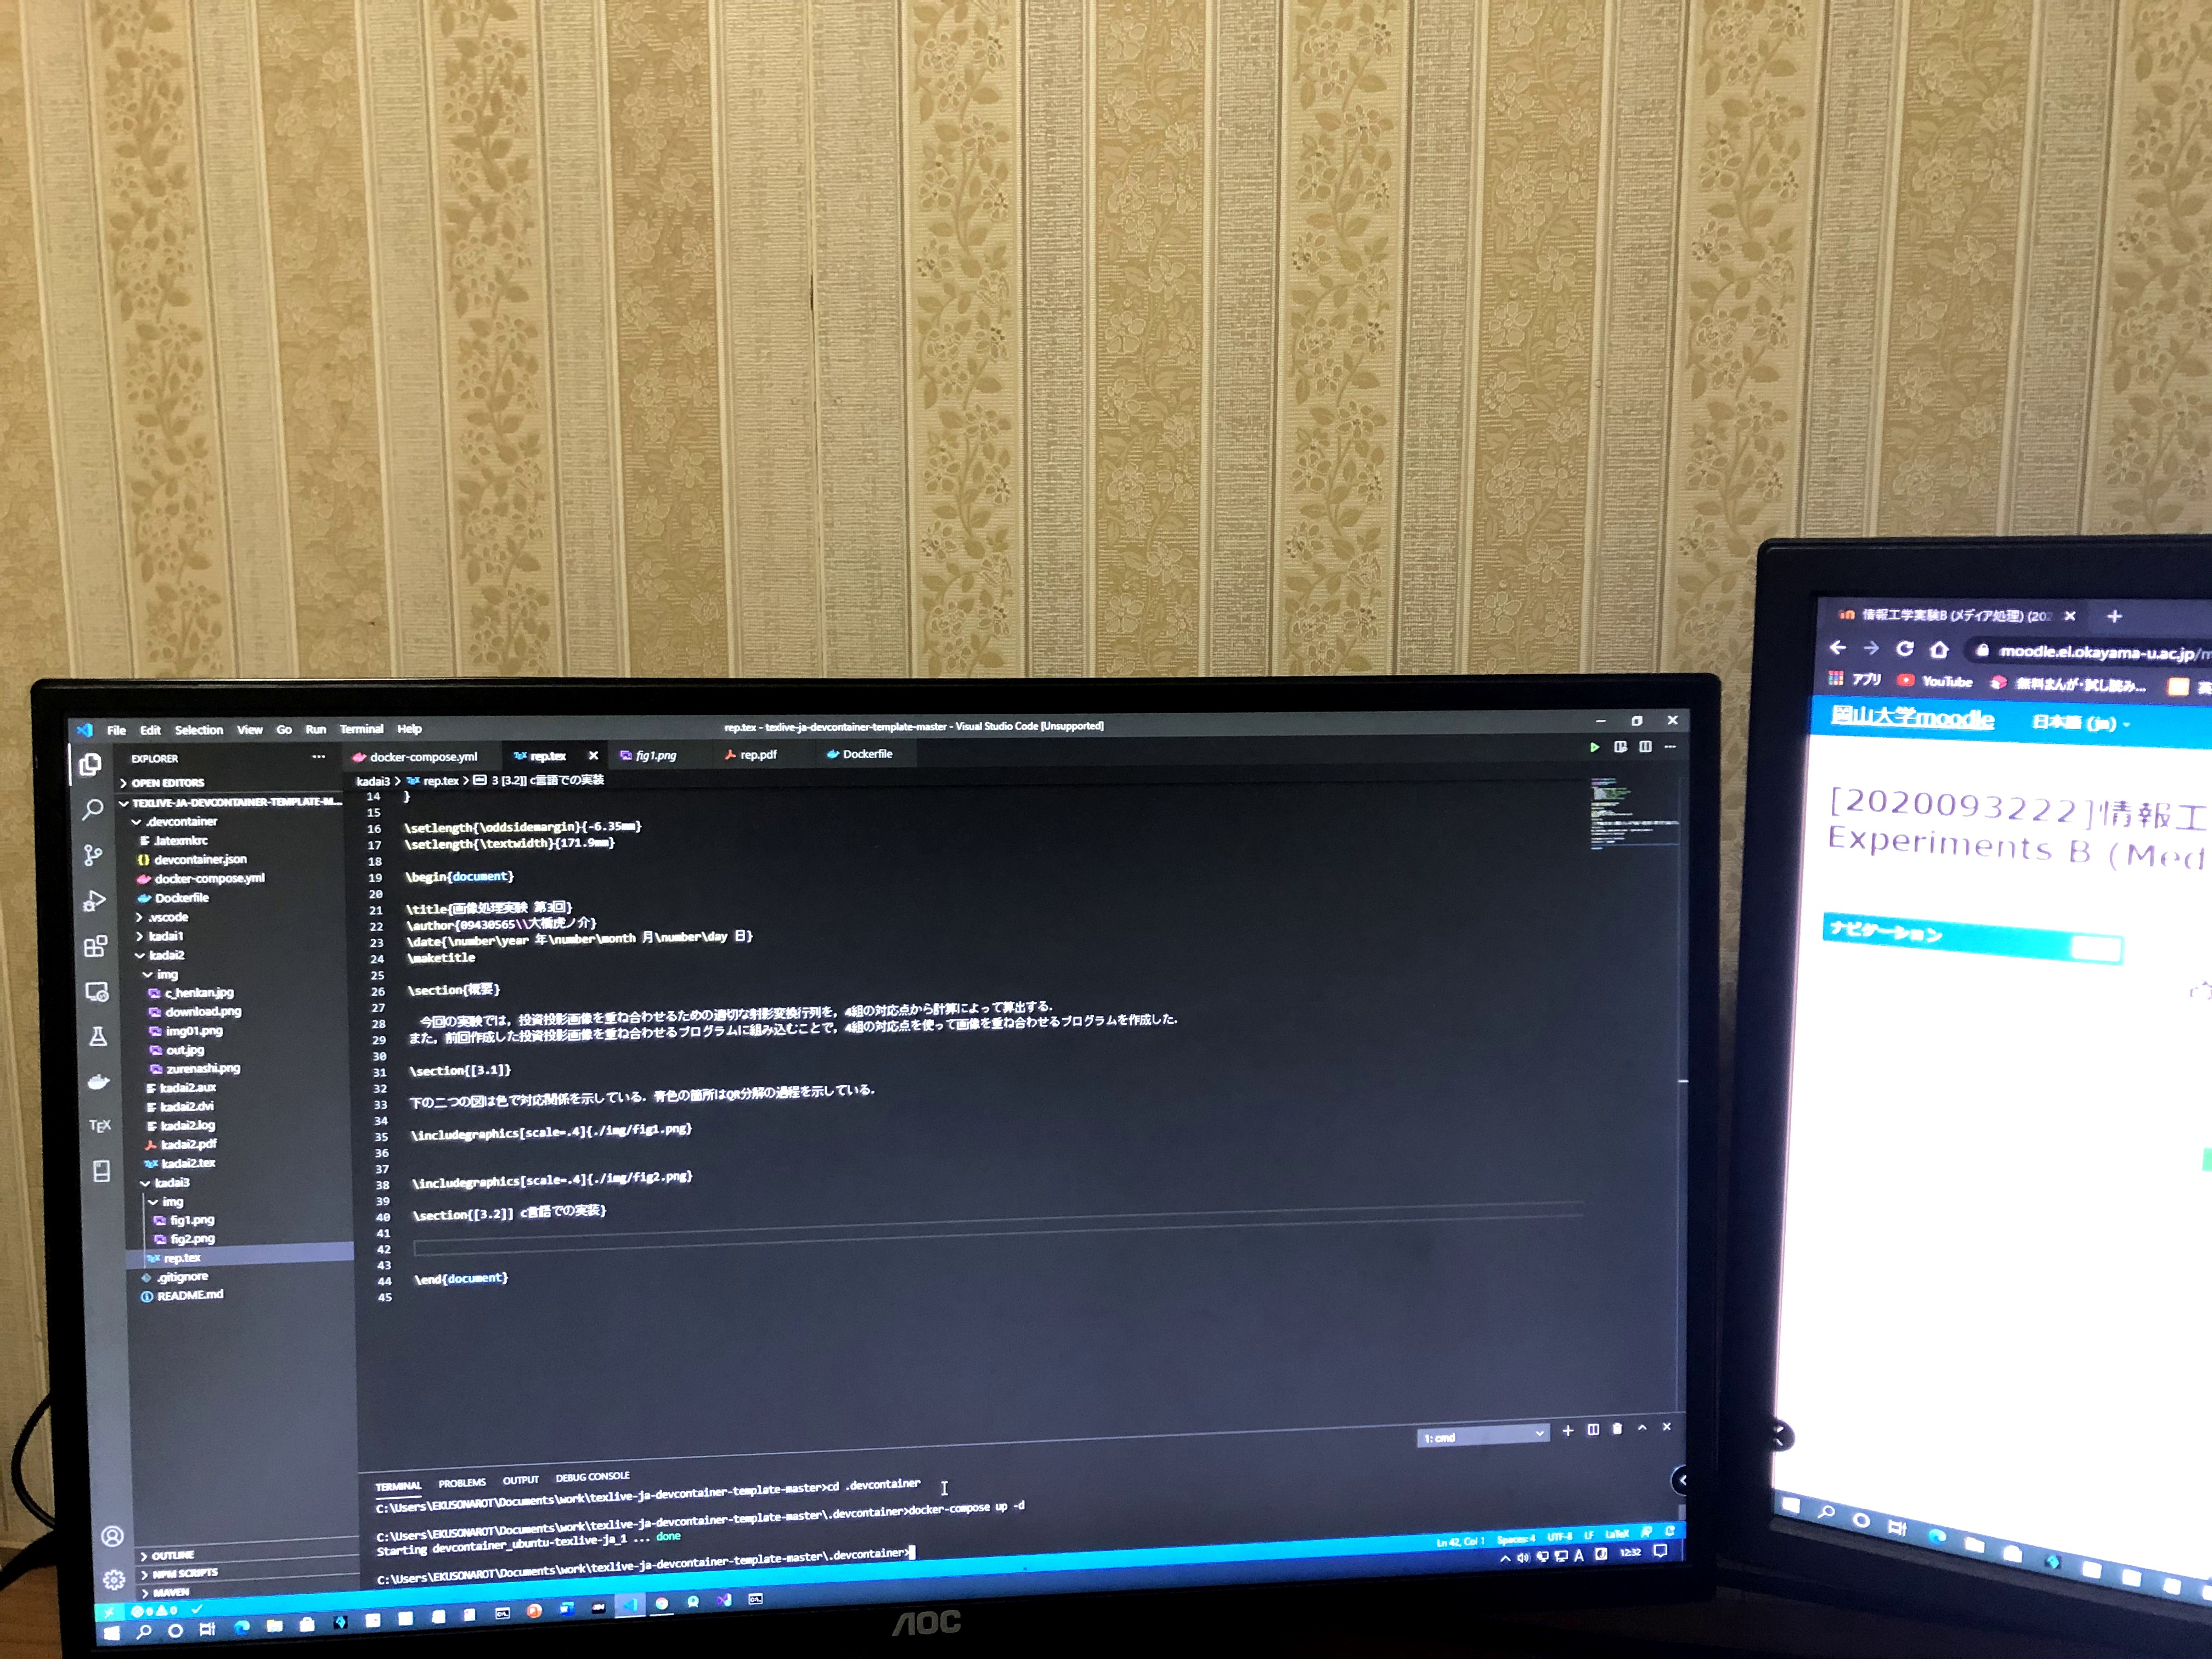
\includegraphics[scale=.055]{./img/desktop1.JPG}

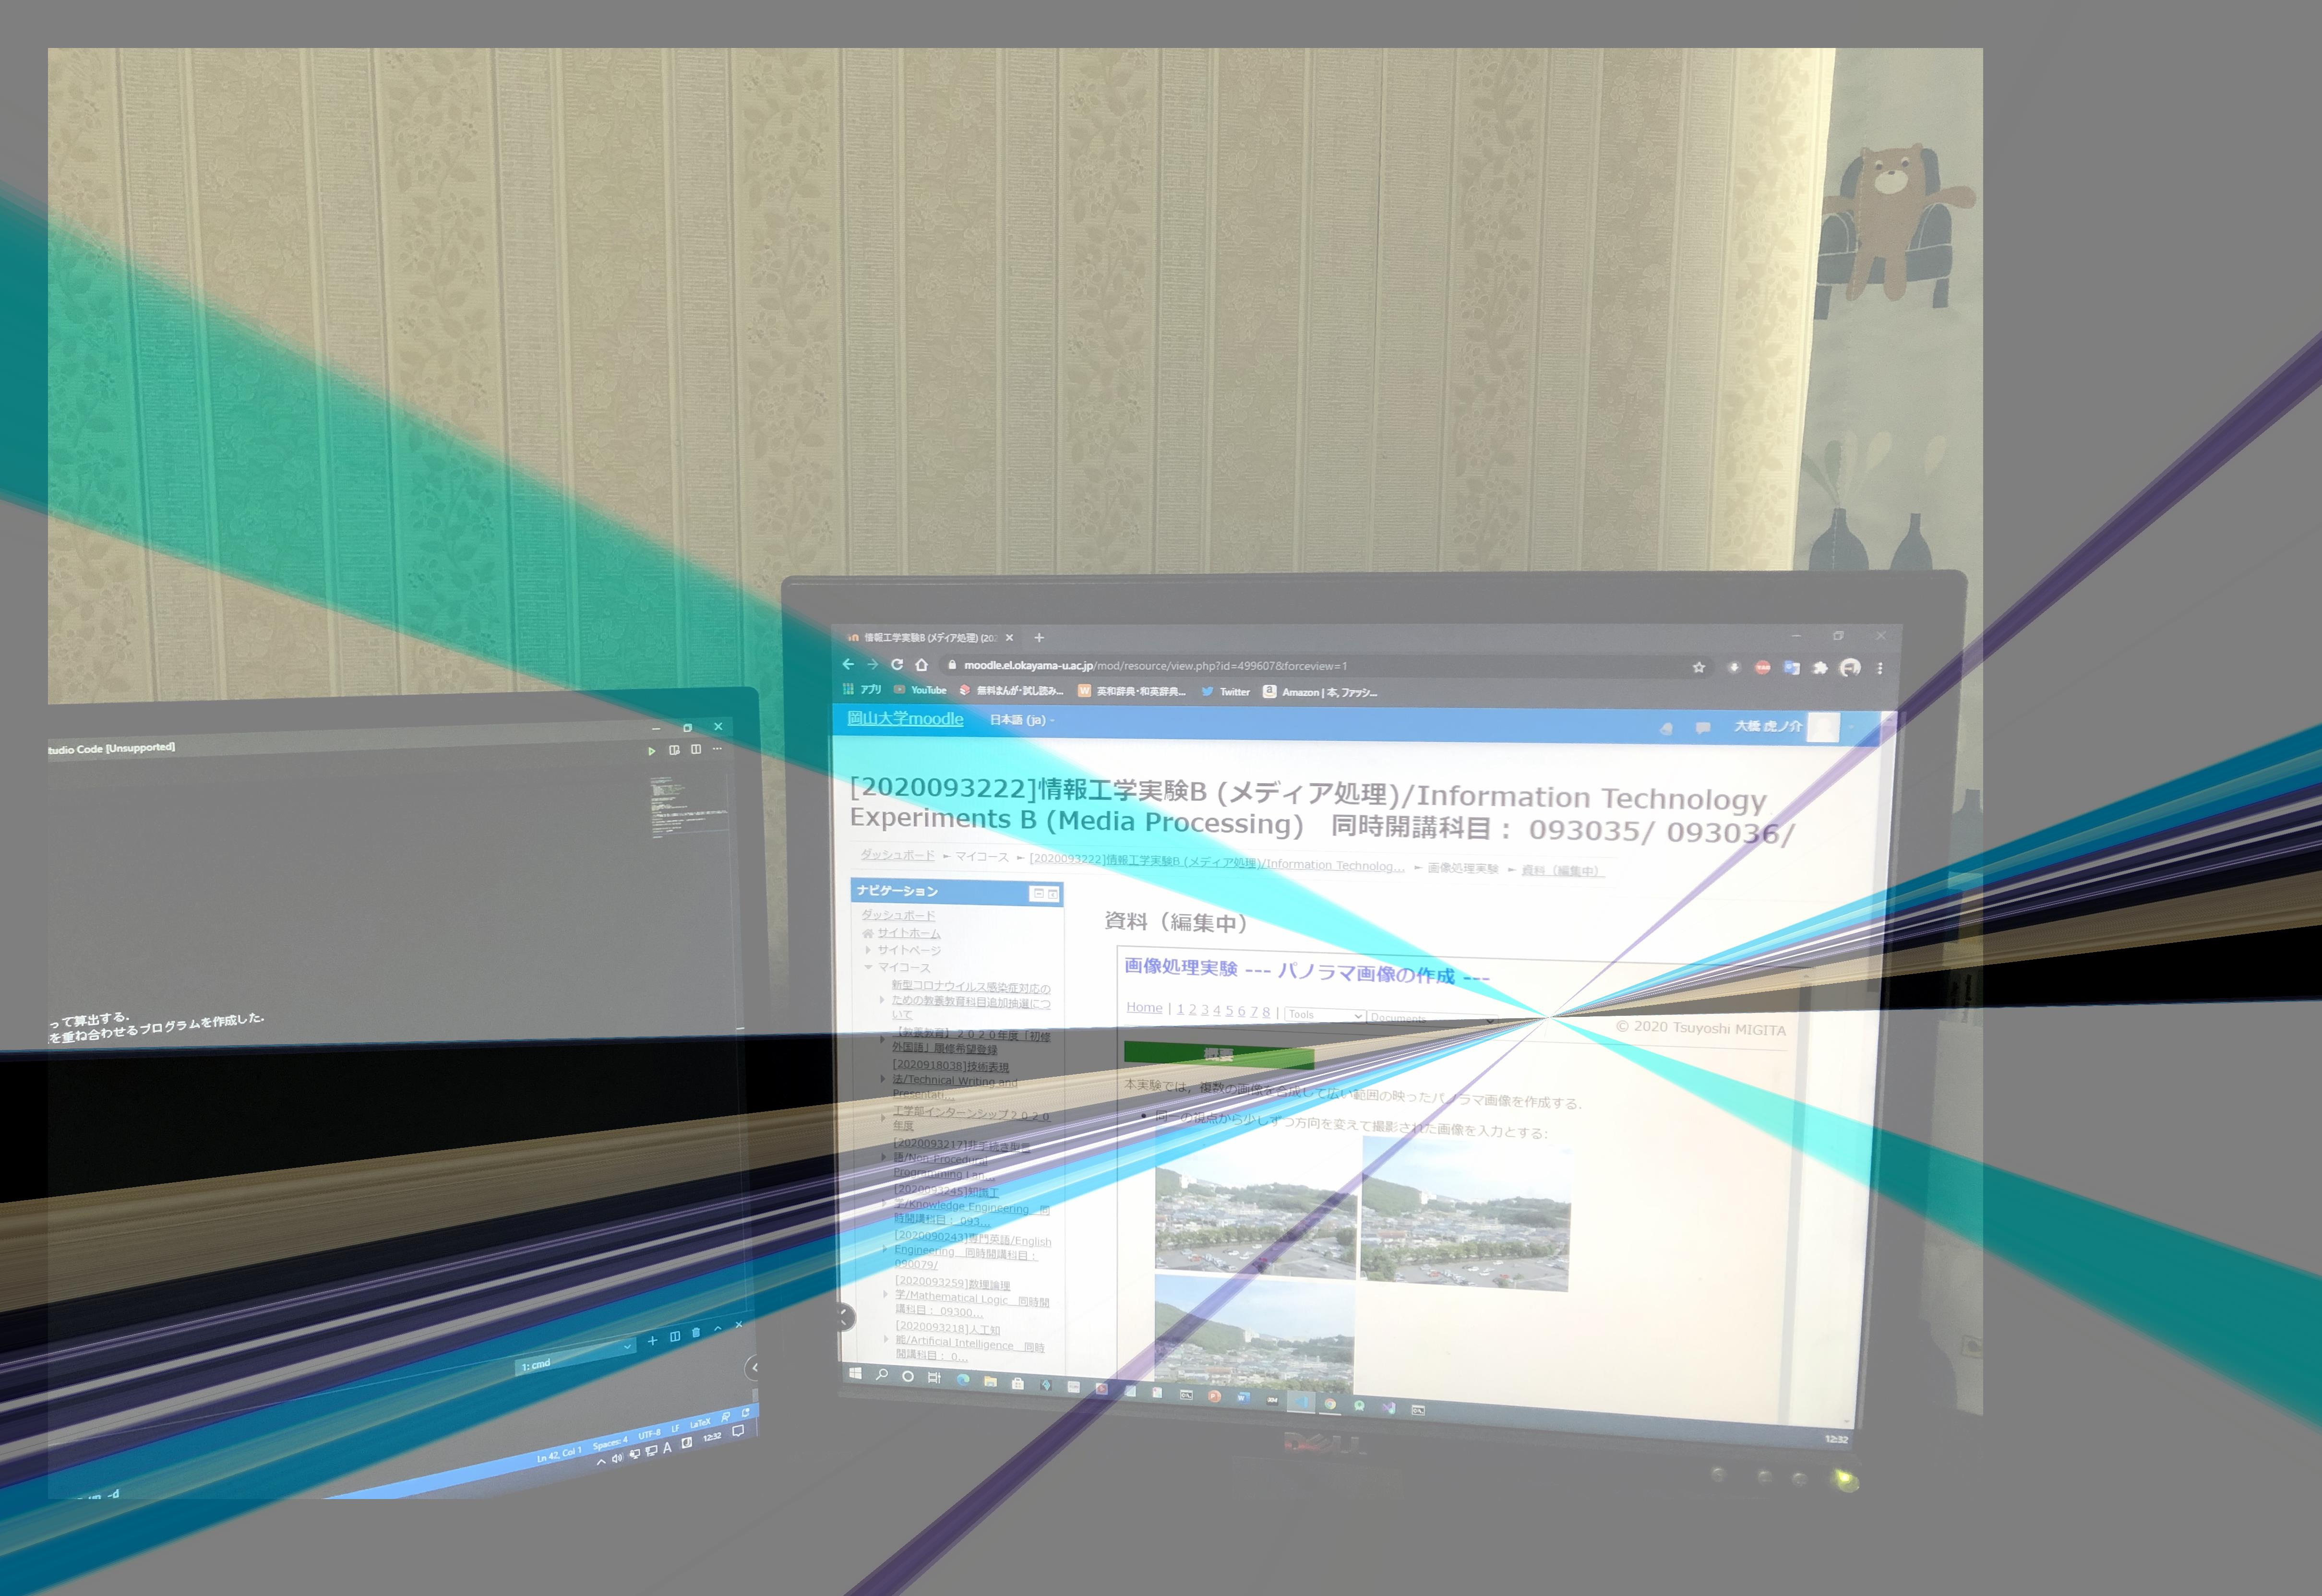
\includegraphics[scale=.11]{./img/desktopout.jpg}

\section{考察}

本報告書では,全8回の実験で実装してきた機能をまとめて自動パノラマ合成プログラム
を作成した結果を報告した.

自分で撮影した画像では正しく合成される画像と正しく合成されない画像があった.
考えられる原因として,正しく合成されない画像は部屋の壁紙が同じパターンの
連続していたためだと考える.仮に,柄のない壁紙であれば,特徴点として記録されないが
上下左右方向に変化がある柄であるために特徴点として扱われ,似たようなパターンが多いため,
正しい特徴点対を探すのが困難であったと考えられる.

今回の実験で工夫した点は,出力画像の大きさを入力画像の大きさによって決めるという点だけであった.
しかし,これでは第1画像と第2画像の重なり具合によって出力画像の大きさを超えてしまう可能性が
ある.なので,射影変換行列と第1画像,第2画像の大きさから出力画像の大きさを計算するのが
最善の方法だと思う.

\end{document}